\chapter{Testing}

\section{Partita single player}
In questo testing sono state verificate:
\begin{itemize}
	\item la creazione random del numero segreto;
	\item la creazione di nuovi livelli;
	\item la segnalazione del livello giocato sul LED a 12 pin;
	\item la corretta rilevazione della distanza sensore-mano;
	\item le tempistiche di accensione del LED RGB corrette;
	\item la variazione dei suoni emessi dal buzzer se si è dentro/fuori il range del lucchetto;
	\item il dimmeraggio/luce fissa del LED verde se si è dentro/fuori il range del lucchetto;
	\item la visualizzazione del numero segreto premendo il button;
	\item la \textbf{routine di fine gioco}:
	\begin{itemize}
		\item carosello dei LED a 12 pin giallo e rosso;
		\item il dimmeraggio temporizzato del LED verde;
		\item la possibilità di avviare l'\textit{easter egg}.
	\end{itemize}
\end{itemize}

Il testing è stato svolto su sistema operativo GNU/Linux \href{https://manjaro.github.io/}{Manjaro}\footnote{Manjaro è una distribuzione GNU/Linux user-friendly basata sullo sviluppato indipendentemente di Arch Linux. All'interno della comunità Linux, Arch è famoso per essere una distribuzione estremamente veloce, potente e leggera che fornisce l'accesso alla versione più recente del software.}.

\begin{figure}[!ht]
	\centering
	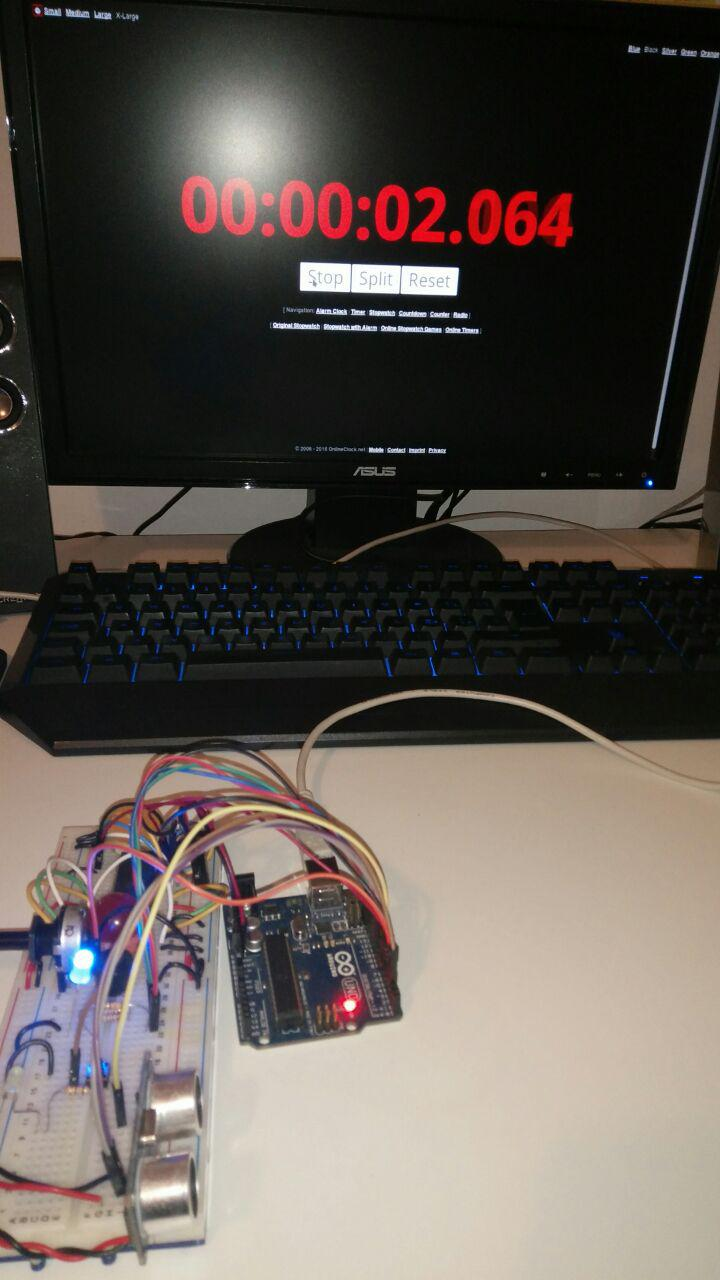
\includegraphics[scale=.25]{img/testing/testing1.jpg}
	\caption{\href{https://youtu.be/X0QOKkfVF4Y}{Testing cronometrato}}
\end{figure}

\clearpage
\section{Web Application - Partita multiplayer}
In questo testing sono state verificate:
\begin{itemize}
	\item la correttezza della comunicazione seriale;
	\item la visualizzazione dello stato dell'avversario.
\end{itemize}

\subsection{Fase di login}
\begin{figure}[!ht]
	\centering
	\begin{subfigure}[b]{0.5\textwidth}
		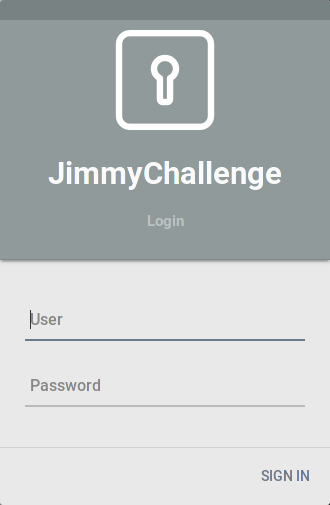
\includegraphics[scale=.4]{img/testing/login.png}
		\caption{Form di login}
	\end{subfigure}
	\begin{subfigure}[b]{0.4\textwidth}
		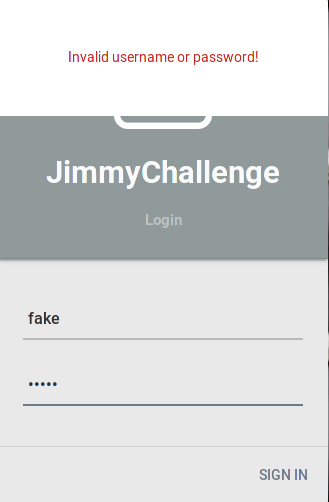
\includegraphics[scale=.4]{img/testing/login_error.png}
		\caption{Errore di login}
	\end{subfigure}
\end{figure}

\clearpage
\subsection{Fase di gioco}
Di seguito sono elencate le fasi di gioco che potrebbero verificarsi.

Per il test da entrambi i giocatori è stato utilizzato il browser Mozilla Firefox e Python 3 su sistema operativo GNU/Linux \href{https://manjaro.github.io/}{Manjaro}.

\begin{figure}[!ht]
	\centering
	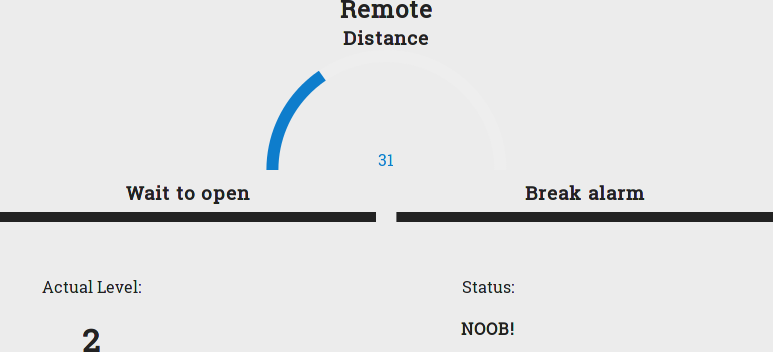
\includegraphics[scale=.4]{img/testing/game1.png}
	\caption{Pistoncino non trovato}
\end{figure}

\begin{figure}[!ht]
	\centering
	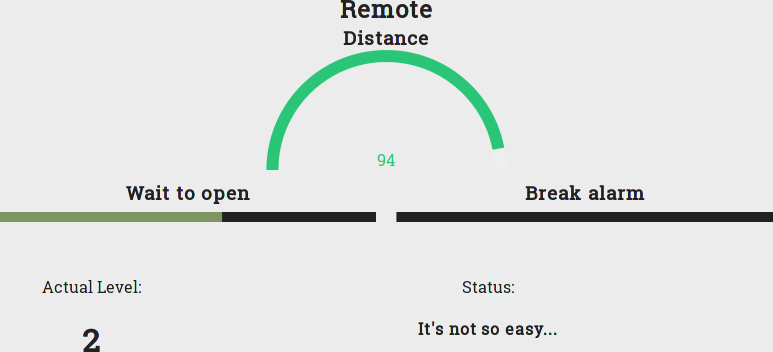
\includegraphics[scale=.4]{img/testing/game2.png}
	\caption{Pistoncino trovato, inizio stato di scasso}
\end{figure}

\begin{figure}[!ht]
	\centering
	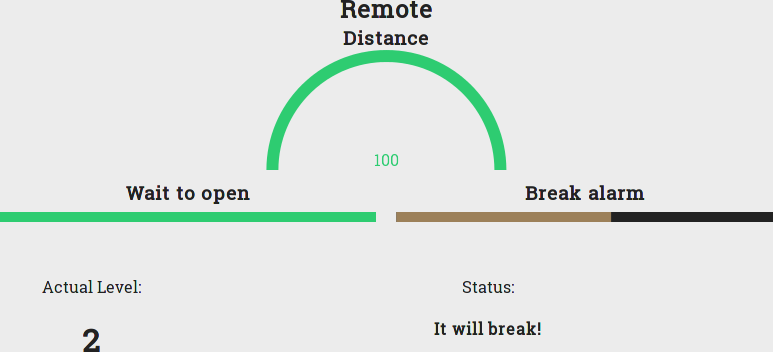
\includegraphics[scale=.4]{img/testing/game3.png}
	\caption{Stato di scasso, rischio rottura}
\end{figure}

\begin{figure}[!ht]
	\centering
	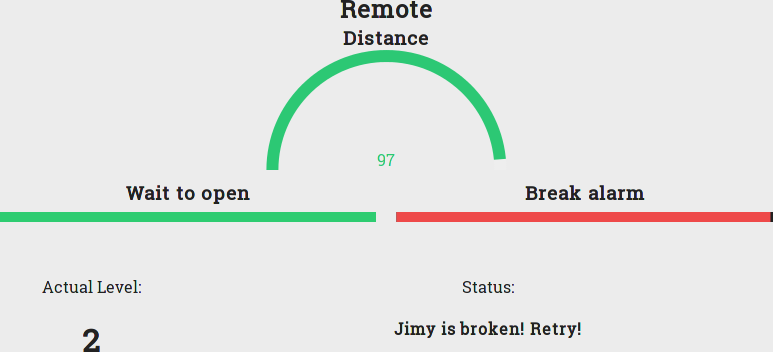
\includegraphics[scale=.4]{img/testing/game4.png}
	\caption{Grimaldello rotto}
\end{figure}

\begin{figure}[!ht]
	\centering
	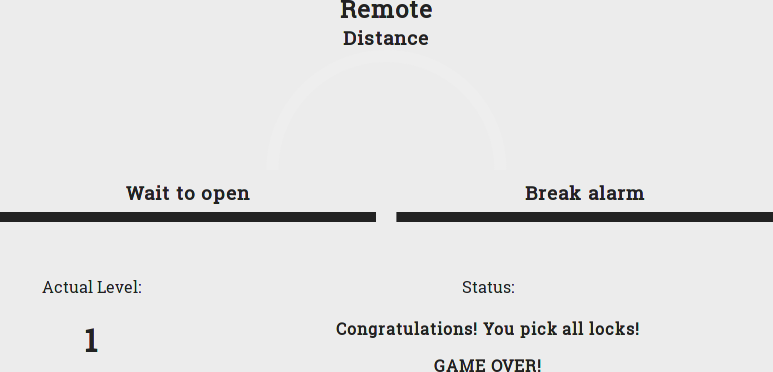
\includegraphics[scale=.4]{img/testing/game5.png}
	\caption{Gioco finito}
\end{figure}

